\chapter{Kravspecifikation} \label{Kravspecifikation}

Kapitlet har til formål, at identificere potentielle kunders ønsker og krav, til en løsning der kan påføre speckle patterns i makroskala, til brug ved DIC. Der differentieres mellem ufravigelige krav og præstationskrav. Løsningen skal overholde de ufravigelige krav, for at den er brugbar. Fra problemformuleringen bliver følgende ufravigelige krav opstillet:
\begin{itemize}
    \item Materialets egenskaber må ikke ændres mere end 1\% efter tilføjelse af speckle pattern (\ref{Optimale speckle patterns}).
    \item Prikker skal deformerer med test-emnet (\ref{Optimale speckle patterns}).
    \item Løsningen skal producere et speckle pattern, der kan anvendes til DIC (\ref{Speckle pattern}).
    \item Løsningen skal kunne placere prikker på en 2D plan overflade (\ref{Afgrænsning}). 
    \item Løsningen skal være en robot (\ref{Robotter}).
\end{itemize}

Præstationskrav har en optimeringsretning, og behøver ikke at være opfyldt før løsningen er funktionel. Løsningen ønskes at have flere eller alle præstationskrav opfyldt, idet præstationskrav baseres på kunders ønsker, øger det konkurrence dygtigheden af den endelige løsning. Præstationskravene udarbejdes gennem House of Quality (HoQ).

%Præstationskravene er krav, som ikke er strengt nødvendige for at produktet virker, men derimod konkurrence punkter.
\plainbreak{2}
\section{House of Quality} \label{House of Quality}
HoQ er et værktøj der benyttes i produktudvikling, til at identificere kunders ønsker og krav til den færdige løsning \parencite{Ullman2018TheProcess}. Det skal sikre, at centrale krav identificeres tidligt i processen og omsættes til målbare tekniske parametre, der kan danne grundlag for en struktureret og velbegrundet udviklingsproces. HoQ er opbygget af 8 trin der er illustreret i figur \ref{fig: HOQ illustration}.  

Udarbejdelsen af et HoQ begynder med trin 1, og fortsætter trin for trin. Udover at identificere kundens ønsker og dertilhørende designspecifikationer, skabes der i trin 6 og 8 indsigt i deres indbyrdes sammenhænge og relationer. Dette tydeliggør de designspecifikationer der er vigtigst at fokusere på, samt eventuelle konflikter eller afhængigheder i designet. Det betyder, at ændringen af én designspecifikation kan have indvirkning på en anden designspecifikation. 

\begin{figure}[H]
    \centering
    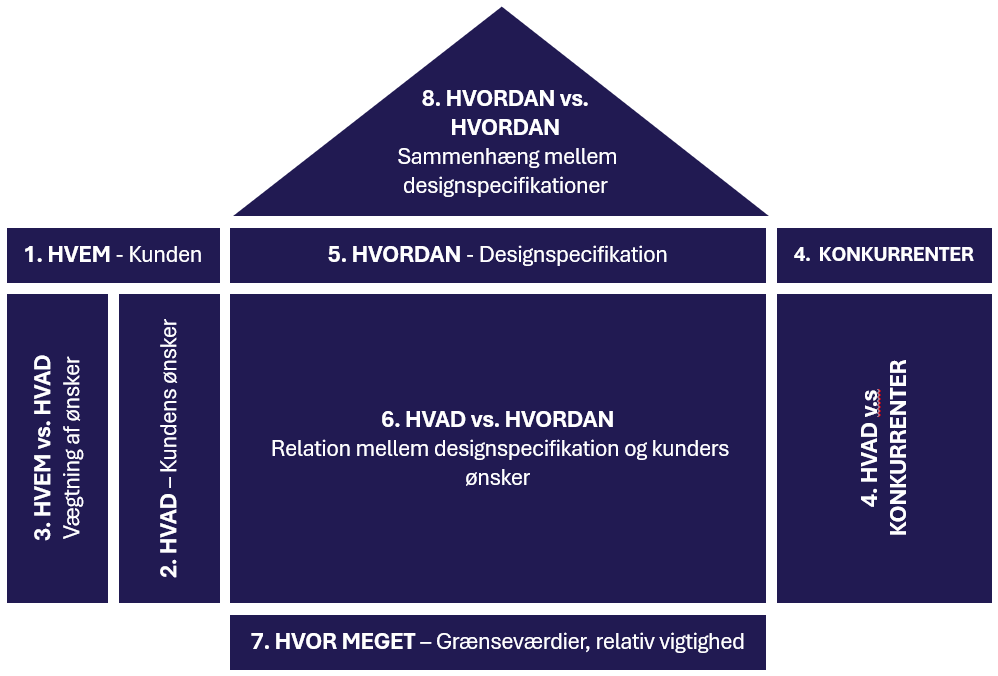
\includegraphics[width=1\linewidth]{Sections/4 Kravspecifikation/Media/HOQ1.png}
    \caption{Illustration af et House of Quality}
    \label{fig: HOQ illustration}
\end{figure} \plainbreak{-0.5}

En væsentlig fordel ved anvendelsen af HoQ er, at metoden bidrager til struktur og systematik i komplekse udviklingsforløb, hvor flere krav og tekniske hensyn skal afvejes. Metoden sikrer desuden en høj grad af klarhed i forhold til, hvordan de opstillede krav afspejles i de valgte designløsninger.



\begin{comment}
\begin{enumerate} 
    \item \textbf{Hvem} - Identifikation af kunder. \\
    \vspace{-0.4cm} \item \textbf{Hvad} - Identifikation af kunders ønsker. \\
    \vspace{-0.4cm} \item \textbf{Hvem vs. hvad} - Vægtning af kundernes ønsker.\\
    \vspace{-0.4cm} \item \textbf{Konkurrenter} - Undersøgelse og evaluering af konkurrenter. \\
    \vspace{-0.4cm} \item \textbf{Hvordan} - Udarbejdelse af designspecifikationer.\\
    \vspace{-0.4cm} \item \textbf{Hvad vs. hvordan} - Relationer mellem designspecifikationer og kundernes ønsker. \\
   \vspace{-0.4cm} \item \textbf{Hvor meget} - Udarbejdelse af grænseværdier for designspecifikationer.\\
\vspace{-0.4cm} \item \textbf{Hvordan vs. hvordan} - Identifikation af designspecifikationernes gensidige afhængighed. \\
\end{enumerate}
\end{comment}

%Processen indledes typisk med en systematisk identifikation af de krav, der vurderes at være væsentlige for det pågældende projekt. Disse krav kan eksempelvis omfatte funktionelle egenskaber, krav til præcision, ydeevne eller andre tekniske specifikationer, der har afgørende betydning for systemets eller produktets samlede funktionalitet. Efterfølgende prioriteres kravene på baggrund af deres betydning, hvorefter de oversættes til konkrete designparametre, som skal sikre opfyldelsen af de ønskede egenskaber.

%HoQ giver et struktureret og visuelt overblik i form af en matrix, hvor relationerne mellem krav og tekniske løsninger tydeliggøres og analyseres. Yderligere skabes der indsigt i, hvordan de tekniske løsninger påvirker hinanden indbyrdes, hvilket muliggør en tidlig identifikation af eventuelle konflikter eller afhængigheder i designet. Herved styrkes beslutningsgrundlaget for udviklingsteamet, som kan foretage prioriteringer med udgangspunkt i en helhedsorienteret vurdering af projektets krav og mål.

%Sammenfattende er HoQ et redskab til at strukturere og kvalificere beslutningsprocesser i projekter, hvor der stilles krav om høj funktionalitet, kvalitet og ydeevne. Metoden giver et solidt fundament for at sikre, at centrale krav bliver integreret i designet, og at de tekniske løsninger udvælges på et velunderbygget grundlag.


\plainbreak{2}
\subsection{Trin 1, 2, 3 og 4 - Identifikation af kunder, ønsker, vægtning og konkurrenter} \label{Trin 1-4}

\textbf{Trin 1} har til formål, at identificerer kunder og interessenter. I dette projekt, er der ingen konkret kunde, så i de følgende trin er kunders ønsker og vægtninger baseret på kapitel \ref{Problemanalyse} Problemanalyse. 
 
\textbf{Trin 2} identificerer kunders ønsker på baggrund af problemanalysen, ved vurdering af, hvad potentielle kunder vægter relevant for en speckle pattern robot. De identificerede ønsker kan ses i tabel \ref{tab: trin 1 til 4} sammen med vægtningen af de enkelte ønsker, som kommer fra trin 3. 

\textbf{Trin 3} vurderer kundens ønsker i forhold til, hvor vigtigt de antages at være baseret på problemanalysen (\ref{Problemanalyse}). Vægtningerne er lavet ved at fordele 100 point mellem de ti ønsker, hvor vigtigere ønsker får tildelt flere point, og mindre vigtige ønsker får tildelt færre point. At begrænse vægtningen til et total på 100 point tvinger en prioritering af ønskerne. 

\renewcommand{\arraystretch}{1.4}
\begin{table}[H]
    \caption{Vægtning af ønsker ved fordeling af 100 point. Vurdering af hvor godt konkurrenter opfylder kundernes ønsker fra fra 0 til 5. 0 = Opfylder overhovedt ikke ønsket, 1 = Minimal opfyldelse af ønsket, 2 = Lille opfyldelse af ønsket, 3 = Tildels opfyldelse af ønsket, 4 = Stor opfyldelse af ønsket og 5 = Fuldstændig opfyldelse af ønsket.}
    \centering
    \begin{tabular}{|l|c||c|c|c|c|} \cline{3-6}\cline{3-6}
    %Konkurrenter
        \multicolumn{2}{c|}{} & \rotatebox{90}{\hspace{-.3cm} \cellcolor{lightgray!20} \textbf{Stempel ruller}} & \rotatebox{90}{\hspace{-.3cm} \cellcolor{lightgray!20} \textbf{Tusch / tegneredskab}}  & \rotatebox{90}{\hspace{-.2cm} \cellcolor{lightgray!20}\textbf{Spraymaling}} & \rotatebox{90}{\hspace{-.3cm} \cellcolor{lightgray!20} \textbf{Midlertidig tatovering} \hspace{.2cm}}\\ 
         
    % Header med Ønsker og vægtning
      \multicolumn{1}{|c}{\cellcolor{aaublue} \textcolor{white}{\textbf{Ønsker}}} & \multicolumn{1}{|c}{\cellcolor{aaublue} \textcolor{white}{\textbf{Vægtning}}} & \multicolumn{4}{|c|}{\cellcolor{aaublue} \textcolor{white}{\textbf{Konkurrenter}}} \\ \specialrule{0pt}{0.5pt}{0pt} \hline 

    %værdier
        1. Producere et godt speckle pattern & 20 & 4 & 3 & 2 & 4\\ \hline
        2. Genskabelighed & 11 & 3 & 0 & 0 & 4 \\ \hline
        3. Håndtere forskellige emnestørrelser og former & 14 & 4 & 5 & 4 & 4 \\ \hline
        4. Håndtere forskellige materialer & 12 & 4 & 4 & 4 & 4 \\ \hline
        5. Hurtig fremstilling af speckle pattern & 10 & 4 & 1 & 5 & 3\\ \hline
        6. Brugervenlighed & 8 & 4 & 5 &3 & 3\\ \hline
        7. Lang levetid & 4 & 4 &1 & 1 & 0\\ \hline
        8. Lav arbejdsbyrde & 14 & 3 & 0 & 3 & 3\\ \hline
        9. Lav førstegangspris & 3 & 1 & 5 & 4 & 2\\ \hline
        10. Lav brugspris & 4 & 3 & 4 & 4 & 3 \\ \hline \specialrule{0pt}{0.8pt}{0pt} \cline{2-6}
        \multicolumn{1}{r|}{\textbf{SUM}} & 100 & 34 & 28 & 30 & 29 \\ \cline{2-6}
    \end{tabular}
    \label{tab: trin 1 til 4}
\end{table} \plainbreak{-0.5}

Det vurderes, at det vigtigste ønske, er ønske 1, om at producere et godt speckle pattern, fordi nøjagtigheden af DIC afhænger af kvaliteten af det anvendte speckle pattern, som det fremgår af afsnit \ref{Speckle pattern}. 

Ønske 3 om håndtering af forskellige emnestørrelse og former, samt ønske 8 om lav arbejdsbyrde tildeles begge 14 point, og er de næstvigtigste ønsker, fordi nuværende metoder til fremstilling af speckle pattern i makroskala, kræver at en person er manuelt involveret under det meste af processen. Det ses derfor som et konkurrencepunkt hvis arbejdsbyrden og tiden kan nedsættes ved automatisering af en robot. På baggrund af afsnit \ref{Fremstilling af Speckle pattern} har ønske 4 om at håndtere forksellige materialer fået 12 point. Dette er grundet DIC i dag anvendes på mange forskellige emnestørrelser og materialer, så det er fordelagtigt, hvis løsningen ikke er begrænset til en enkelt emnestørrelse eller materiale. 

De sidste ønsker, som ikke er nævnt, har en mindre vægtning. De er derfor ikke lige så relevante som de nævnte ønsker, og deres vægtning bliver dermed ikke forklaret yderligere. Alle vægtningerne kan ses i figur \ref{tab: trin 1 til 4}.


\textbf{Trin 4} ses til højre i tabel \ref{tab: trin 1 til 4}, hvor konkurrenterne vurderes på baggrund af ønskerne. Vurderingen af konkurrenter sker, for at identificerer ønsker, hvor der er mulighed for at skabe konkurrencepunkter. Fra afsnit \ref{Fremstilling af Speckle pattern} er stempel ruller, tusch/tegneredskab, spraymaling og midlertidig tatovering valgt som konkurrenter. Disse vægtes på en skala fra 0 til 5: %, disse kan ses i tabel \ref{...}:


\newcommand{\myhash}{\raisebox{\depth}{\#}}
\begin{enumerate}[font=\bfseries]\addtocounter{enumi}{-1}
    \item Opfylder overhovedet ikke ønsket 
    \item Minimal opfyldelse af ønsket 
    \item Lille opfyldelse af ønsket 
    \item Tildels opfyldelse af ønsket 
    \item Stor opfyldelse af ønsket 
    \item Fuldstændig opfyldelse af ønsket 
\end{enumerate}


Vurdering af konkurrenterne sker på baggrund af afsnit \ref{Fremstilling af Speckle pattern} i problemanalysen. Stempelruller og midlertidig tatoveringer får begge 4 point i ønske 1, hvor de øvrige får mindre. Dette betyder, at en endelig løsning helst skal have $\geq 4$, medmindre løsningen excellerer på andre områder, fordi ønsket har fået 20 point. Konkurrenterne får henholdsvis 3, 0, 3 og 3 point i ønske 8 om lav arbejdsbyrde, som er det ønske der vægtes anden højest. Det vurderes derfor, at lav arbejdsbyrde er et af de områder, som en løsningen kan differentiere sig fra konkurrenterne på. Det forventes at førstegangsprisen og brugsprisen af en robot som løsning, overstiger både tuscher og spraymaling. Løsningen vil stadig have markedspotentiale, da disse ønsker er vurderet lavest. 

 



\begin{comment}
Tidligere tabeller:

  \begin{table}[H]
    \caption{Vægtede ønsker}
    \centering
    \begin{tabular}{|l|c|}\hline
     \multicolumn{1}{|c}{\cellcolor{aaublue} \textcolor{white}{\textbf{Ønsker}}} &  \multicolumn{1}{|c}{\cellcolor{aaublue} \textcolor{white}{\textbf{Vægtning (ud af 100)}}} \\ \specialrule{0pt}{0.5pt}{0pt} \hline 
        1. Producere et godt speckle pattern & 20 \\ \hline
        2. Genskabelighed & 11\\ \hline
        3. Håndtere forskellige emnerstørrelser og former & 13 \\ \hline
        4. Håndtere forskellige materialer & 13 \\ \hline
        5. Hurtig fremstilling af speckle pattern & 10\\ \hline
        6. Brugervenlighed & 8\\ \hline
        7. Lang levetid & 4\\ \hline
        8. Lav arbejdsbyrde & 14 \\ \hline
        9. Lav førstegangspris & 3\\ \hline
        10. Lav brugspris & 4\\ \hline
    \end{tabular}
    \label{tab:vægønsker}
\end{table} 



\begin{table}[H]
    \centering
    \caption{Kundens vurdering af konkurrenternes produkter}
    \renewcommand{\arraystretch}{1.3} 
    \setlength{\tabcolsep}{8pt} 
    \begin{tabular}{|l|c|c|c|c|c|c|c|c|c|c||c|}
        \hline
        \rowcolor{lightgray!20} \cellcolor{aaublue}\textcolor{white}{ \textbf{ Ønske nr.}} & \textbf{1} & \textbf{2} & \textbf{3} & \textbf{4} & \textbf{5} & \textbf{6} & \textbf{7} & \textbf{8} & \textbf{9} & \textbf{10} & \textbf{sum} \\ \hline 
        \specialrule{0pt}{0.5pt}{0pt} \hline 
        
        \multicolumn{1}{|l|}{\cellcolor{aaublue} \textcolor{white}{\textbf{Stempel ruller}}} & 4 & 3 & 4 & 4 & 4 & 4 & 4 & 3 & 1 & 3 & 34 \\ 
        \hline
         \multicolumn{1}{|l|}{\cellcolor{aaublue} \textcolor{white}{\textbf{tusch / tegneredskab}}} & 3 & 0 & 5 & 4 & 1 & 5 & 1 & 0 & 5 & 4 & 28 \\ 
        \hline
        \multicolumn{1}{|l|}{\cellcolor{aaublue} \textcolor{white}{\textbf{Spraymaling}}} & 2 & 0 & 4 & 4 & 5 & 3 & 1 & 3 & 4 & 4 & 30 \\ 
        \hline
        \multicolumn{1}{|l|}{\cellcolor{aaublue} \textcolor{white}{\textbf{Midlertidig tatovering}}}  & 4 & 4 & 4 & 4 & 3 & 3 & 0 & 3 & 1 & 3 & 29 \\ 
        \hline
    \end{tabular}
    \label{Tab: Kunde vs. konk.}
\end{table}


\begin{table}[H]
    \caption{Vægtede ønsker fra 0 til 100}
    \centering
    \begin{tabular}{|l|c | p{.1pt}|c|c|c|c|} \cline{4-6}\cline{4-7}
    %Konkurrenter
        \multicolumn{3}{c|}{}  & \rotatebox{90}{\hspace{-.3cm} \cellcolor{lightgray!20} \textbf{Stempel ruller}} & \rotatebox{90}{\hspace{-.3cm} \cellcolor{lightgray!20} \textbf{tusch / tegneredskab}}  & \rotatebox{90}{\hspace{-.2cm} \cellcolor{lightgray!20}\textbf{Spraymaling}} & \rotatebox{90}{\hspace{-.2cm} \cellcolor{lightgray!20}\textbf{Midlertidig tatovering}}\\ 
         
    % Header med Ønsker og vægtning
      \multicolumn{1}{|c}{\cellcolor{aaublue} \textcolor{white}{\textbf{Ønsker}}} & \multicolumn{1}{|c}{\cellcolor{aaublue} \textcolor{white}{\textbf{Vægtning}}} & ~ & \multicolumn{4}{|c|}{\cellcolor{aaublue} \textcolor{white}{\textbf{Konkurrenter}}} \\ \specialrule{0pt}{0.5pt}{0pt} \cline{1-2} \cline{4-7}

    %værdier
        1. Producere et godt speckle pattern & 20 & ~ &  4 & 3 & 2 & 4\\ \cline{1-2} \cline{4-7}
        2. Genskabelighed & 11 & ~ & 3 & 0 & 0 & 4 \\ \cline{1-2} \cline{4-7}
        3. Håndtere forskellige emnerstørrelser og former & 13 & ~ & 4 & 5 & 4 & 4 \\ \cline{1-2} \cline{4-7}
        4. Håndtere forskellige materialer & 13 &  ~& 4 & 4 & 4 & 4 \\ \cline{1-2} \cline{4-7}
        5. Hurtig fremstilling af speckle pattern & 10 &  ~& 4 & 1 & 5 & 3\\ \cline{1-2} \cline{4-7}
        6. Brugervenlighed & 8 &  ~& 4 & 5 &3 & 3\\ \cline{1-2} \cline{4-7}
        7. Lang levetid & 4 & ~ & 4 &1 & 1 & 0\\ \cline{1-2} \cline{4-7}
        8. Lav arbejdsbyrde & 14 &  ~&3 & 0 & 3 & 3\\ \cline{1-2} \cline{4-7}
        9. Lav førstegangspris & 3 & ~ & 1 & 5 & 4 & 2\\ \cline{1-2} \cline{4-7}
        10. Lav brugspris & 4 & ~ & 3 & 4 & 4 & 3 \\ \cline{1-2} \cline{4-7} \specialrule{0pt}{0.8pt}{0pt} \cline{4-7}
        \multicolumn{3}{r|}{\textbf{SUM}}  & 34 & 28 & 30 & 29 \\ \cline{4-7}
    \end{tabular}
    \label{tab: trin 1 til 4}
\end{table}
\end{comment} \plainbreak{2}
\subsection{Trin 5 - Udarbejdelse af designspecifikationer} \label{Trin 5}
Det femte trin har til formål, at omsætte ønsker til målbare designspecifikationer, der muligører konkrete og målbare test af den endelige løsning. Designspecifikationerne beskrives i dette afsnit og kan ses i tabel \ref{tab:krav}.

\renewcommand{\arraystretch}{1.2}
\begin{table}[H]
    \centering
     \caption{Design specifikationer.For optimerings retningen (OR) betyder \textbf{--} en fastlagt værdi, \protect$\btdown$ betyder specifikationen forbedres når værdien mindskes og $\blacktriangle$ betyder specifikationen forbedres når værdien øges}
    \begin{tabular}{|l|c|c|} \hline
     \multicolumn{1}{|c}{\cellcolor{aaublue} \textcolor{white}{\textbf{Designspecifikation}}} &  \multicolumn{1}{|c}{\cellcolor{aaublue} \textcolor{white}{\textbf{Enhed}}} &  \multicolumn{1}{|c}{\cellcolor{aaublue} \textcolor{white}{\textbf{OR}}} \\ \specialrule{0pt}{0.5pt}{0pt} \hline 
        1. Prikstørrelse& mm & \textbf{--} \\ \hline
        2. Variation på prikstørrelser & mm & $\btdown$ \\ \hline
        3. Variation på prikplacering & mm & $\btdown$ \\ \hline
        4. Størrelse af arbejdsområdet & mm & $\blacktriangle$\\ \hline
        5. Flytning af emnet under fremstilling af speckle pattern & mm & $\btdown$\\ \hline
        6. Antal forskellige farvemidler til speckle pattern & Farvemidler & $\blacktriangle$ \\ \hline
        7. Kontrast mellem prik og baggrund	& -- & $\blacktriangle$ \\ \hline
        8. Tidsforbrug på prikplacering & $\SI{}{s/cm^2}$ & $\btdown$ \\ \hline
        9. Brugerinvolvering under process & min & $\btdown$\\ \hline
        10. Tid brugt på opsætning  & min & $\btdown$\\ \hline
        11. Antal værktøj til at samle hele produktet & Værktøj & $\btdown$ \\ \hline
        12. Antal specialværktøj til at samle hele produktet & Værktøj & $\btdown$\\ \hline
    \end{tabular}
    \label{tab:krav}
\end{table}

\textbf{1. Prikstørrelse} er valgt på baggrund af ønske 3 om forskellige emnestørrelser og former. Denne designspecifikation beskriver det spænd af prikstørrelser løsningen kan producere. 

\textbf{2. Variation på prikstørrelser} beskriver den acceptable afvigelse fra den valgte prikstørrelse. For at kunne producere et godt speckle pattern skal denne variation minimeres.

\textbf{3. Variation af prikplacering} beskriver den acceptable afvigelse fra den teoretiske placering og den virkelige placering. Dette er valgt på baggrund af den høje vægtning tildelt ønske 2 om genskabelighed. 

\textbf{4. Størrelse af arbejdsområdet} sættes som designspecifikation, fordi det skal være muligt, at sætte prikker på forskellige størrelser emner, som det fremgår af ønske 3. 

\textbf{5. Fastholdelse af emnet} sikrer et godt speckle pattern som der vægtes i ønske 1. Det er en nødvendighed, at emnet ikke bevæger sig under påføring, således robotten kan overføre det ønskede speckle pattern så præcist som muligt.

\textbf{6. Antal forskellige farvemidler til speckle pattern} skal sikre, at produktet kan skabe speckle patterns på alle emnematerialer ved at inkludere flere forskellige farvemidler, så farver og materialer altid fungere optimalt i forhold til det enkelte emne.

\textbf{7. Kontrast mellem prik og baggrund} er en nødvendighed for at have et godt speckle pattern, som der ønskes i ønske 1. Det beskriver forholdet i lysstyrke mellem prik og emnet.

\textbf{8. Tidsforbrug på prikplacering} kommer direkte fra ønske 5 om hurtig fremstilling af speckle patterns. 

\textbf{9. Brugerinvolvering under proces} specificeres som den mængde tid, brugeren skal bruge efter de har sat processen i gang. Dette skal minimeres for at opfylde ønske 6 samt 8. En løsning der kræver at brugeren observerer den under processen er ikke brugervenlig.
  
\textbf{10. Tid brugt på opsætning} er en faktor i ønske 6 og 8. Dette beskriver tiden brugt på at sætte processen i gang.

\textbf{11. Antal værktøj til at samle hele produktet} har en effekt på hvor intuitiv løsningen er at samle. For at lave produktet brugervenligt, ønskes antallet derved så lavt som muligt.

\textbf{12. Antal specialværktøj til at samle hele produktet} er til for at holde løsningen brugervenlig som mulig, da løsningen ikke skal blive unødvendigt krævende at sammensætte. Derfor fremsættes en øvre grænse for, hvor mange forskellige stykker specialværktøj, der må påkræves for at samle produktet.

\plainbreak{2}
\subsection{Trin 6 - Relationer mellem designspecifikationer og kundernes ønsker} \label{Trin 6}
I det 6. trin beskrives relationen mellem kundens ønsker og de udarbejdede designspecifikationer. Her er der givet henholdsvis 1 point for en lav relation $(\bigtriangledown)$, 3 point for en middel relation $(\bigcirc)$ og 9 point for en stærk relation $(\blackbigcirc)$.  Det efterstræbes at alle ønsker som minimum har én stærk relation til 2 designspecifikationer, som det ses i tabel 4.3 i trin 6. Herved sikres, at ønskerne er ligeligt repræsenteret i designspecifikationerne.

\begin{table}[H]
\centering
\caption{ Relation mellem ønsker og designspecifikationer. $\protect\blackbigcirc$ = stærk relation, $\bigcirc$ = moderat relation og $\bigtriangledown$ = svag relation.}
\label{fig: HOQ trin 6} 
\footnotesize
\def\arraystretch{2}
\begin{tabular}{|p{4.cm}|c|c|c|c|c|c|c|c|c|c|c|c|}
    \hline
    \cellcolor{aaublue} \textcolor{white}{\diagbox[height=6cm, width=4.4cm]{\raisebox{0.9\height}{\enspace \textbf{\large Ønsker}}}{\raisebox{-0.9\height}{\enspace \makecell{\textbf{\normalsize Design-} \\ \textbf{\normalsize Specifikationer}}}}} & \cellcolor{lightgray!20} \rotatebox{90}{\hspace{-2.9cm} 1. Prikstørrelse} & \cellcolor{lightgray!20} \rotatebox{90}{\hspace{-2.9cm} 2. Variation på prikstørrelse} & \cellcolor{lightgray!20} \rotatebox{90}{\hspace{-2.9cm} 3. Variation på prikplacering} & \cellcolor{lightgray!20} \rotatebox{90}{\hspace{-2.9cm} 4. Størrelse af arbejdsområde} & \cellcolor{lightgray!20} \rotatebox{90}{\hspace{-2.9cm} \makecell[l]{\addlinespace[-3pt] 5. FLytning af emnet under fremstilling \\ \quad af speckle pattern \vspace{-3pt} }} & \cellcolor{lightgray!20} \rotatebox{90}{\hspace{-2.9cm} \makecell[l]{\addlinespace[-3pt] 6. Antal forskellige farvemidler til \\ \quad speckle pattern \vspace{-3pt}}} & \cellcolor{lightgray!20} \rotatebox{90}{\hspace{-2.9cm} \makecell[l]{\addlinespace[-3pt] 7. Kontrast mellem prik og baggrund \vspace{-3pt} }} & \cellcolor{lightgray!20} \rotatebox{90}{\hspace{-2.9cm} 8. Tidsforbrug på prikplacering} &\cellcolor{lightgray!20} \rotatebox{90}{\hspace{-2.9cm} 9. Brugerinvolvering under process} & \cellcolor{lightgray!20} \rotatebox{90}{\hspace{-2.9cm} 10. Tid brugt på opsætning} & \cellcolor{lightgray!20} \rotatebox{90}{\hspace{-2.9cm} \makecell[l]{\addlinespace[-3pt] 11. Antal værktøj til at samle hele \\ \quad produktet }} & \cellcolor{lightgray!20} \rotatebox{90}{\hspace{-2.9cm} \makecell[l]{\addlinespace[-3pt] 12. Antal specialværktøj til at samle \\ \quad hele produktet \vspace{-3pt} }}  \\
    \hline
     \cellcolor{lightgray!20} \makecell[l]{\addlinespace[0pt] 1. Producere et godt \\ \quad speckle pattern \vspace{0pt}} & $\bigcirc$ & $\blackbigcirc$ & $\blackbigcirc$ & & $\blackbigcirc$  &  & $\bigcirc$ &  & & & & \\
    \hline
    \cellcolor{lightgray!20} 2. Genskabelighed & $\bigtriangledown$& $\blackbigcirc$ & $\blackbigcirc$ & & $\blackbigcirc$& & & & & &&\\
    \hline
    \cellcolor{lightgray!20} \makecell[l]{\addlinespace[0pt] 3. Håndtere forskellige \\ \quad objekt størrelser og former} \vspace{-10pt}  & $\blackbigcirc$& & & $\blackbigcirc$ &$\bigcirc$& & &$\bigcirc$& & & &\\
    \hline
    \cellcolor{lightgray!20} \makecell[l]{\addlinespace[0pt] 4. Håndtere forskellige \\ \quad materialer} \vspace{0pt} & & & & & $\bigcirc$ & $\blackbigcirc$& $\blackbigcirc$ & & & & & \\
    \hline
    \cellcolor{lightgray!20} \makecell[l]{\addlinespace[0pt]  5. Hurtig fremstilling af \\ \quad speckle pattern} \vspace{0pt} & $\bigcirc$& $\bigtriangledown$&$\bigtriangledown$& $\bigcirc$ & & &  & $\blackbigcirc$ & $\bigcirc$ & $\blackbigcirc$& & \\
    \hline
    \cellcolor{lightgray!20} 6. Brugervenlighed && & & & & & & & $\bigtriangledown$& $\bigcirc$ & $\blackbigcirc$ & $\blackbigcirc$ \\
    \hline
    \cellcolor{lightgray!20} 7. Lang levetid & & & & & & $\bigcirc$ & & $\bigtriangledown$& & &$\blackbigcirc$& $\bigcirc$ \\
    \hline
    \cellcolor{lightgray!20} 8. Lav arbejdsbyrde & & & & & & & & & $\blackbigcirc$ & $\blackbigcirc$ & $\bigcirc$& $\bigcirc$\\
    \hline
    \cellcolor{lightgray!20}  9. Lav førstegangspris&$\bigcirc$& $\bigcirc$& $\bigcirc$& $\bigcirc$& &$\bigcirc$ & & $\blackbigcirc$& & & & $\blackbigcirc$ \\
    \hline
    \cellcolor{lightgray!20} 10. Lav brugspris& & & & & & $\blackbigcirc$ & & & $\bigcirc$& $\blackbigcirc$& &  \\
    \hline
\end{tabular}
\end{table} \plainbreak{-0.5}

Relationer mellem ønsker og designspecifkationer kan være positive, såvel som negative. Design specifikation 2 og 3 for eksempel har en positiv relation med ønsket om genskabelighed, men en negativ relation med ønsket om lav førstegangspris. For at skabe en høj genskabelighed skal produktet have en høj nøjagtighed. En forøgelse af nøjagtighed (og dermed lavere tolerancer) kommer ofte også med en højere pris. Dermed modstrider disse ønsker hinanden. Dette uddybes i afsnit \ref{Trin 8}.
\plainbreak{2}
\subsection{Trin 7 - Udarbejdelse af grænseværdier for designspecifikationer} \label{Trin 7} 

Designspecifikationer er målbare krav, med en optimerings retning og en grænseværdi. Grænseværdierne opstilles for designspecifikationerne fra tabel \ref{tab:krav}, på baggrund af problemanalysen i kapitel \ref{Problemanalyse}. Løsninger der ligger udenfor én eller flere af grænseværdierne, er ikke konkurrencedygtige på de punkter, men er stadig funktionelle løsninger.

Designspecifikation 1 har ingen optimeringsretning, fordi den har en øvre og en nedre grænse. Den nedre grænse er en hård grænse da løsningen vil bevæge sig ind i mikroskala-området hvis den kommer under. Den beskrives som en designspecifikation, da en løsning der kun kan producere prikker mellem \(\SI{0,1}{mm}\) og \(\SI{0,5}{mm}\) stadig er en funktionel løsning, men den mister konkurrencedygtighed. Herunder sættes værdier og enheder på designspecifikationerne.

%Designspecifikation 1 er unik i forhold til de andre da den ingen optimeringsretning har, og reelt består af 2 forskellige værdier, en øvre og nedre grænse. 

%For designspecifikation 1 er den ønskede specifikation angivet til mellem 0,1 og 1. Der er ingen optimeringsretning, idet prikstørrelsen skal være valgbar indenfor det ønskede interval. Der er afgrænset til makroskala, hvorfra grænseværdien er $\leq 0.1$ mm, som angiver grænsen mellem mikro- og makroskala. Et produkt der producerer prikker på mikroskala opfylder ikke kravet om makroskala, og kan derfor ikke anvendes til det ønskede formål. Der opstilles ønskede specifikationer for alle designspecifikationer, som ses i tabel \ref{tab:trin 7 designspec}.  


\begin{table}[H]
    \centering
     \caption{Design specifikationer. For optimerings retningen (OR) betyder \textbf{--} en fastlagt værdi, \protect$\btdown$ betyder specifikationen forbedres når værdien mindskes og $\blacktriangle$ betyder specifikationen forbedres når værdien øges. Relativ vigtighed ($\Omega$)}
      \begin{tabular}{|l|c|c|c|c|} \hline
     \multicolumn{1}{|c}{\cellcolor{aaublue} \textcolor{white}{\textbf{Designspecifikation}}} & \multicolumn{1}{|c}{\cellcolor{aaublue} \textcolor{white}{\textbf{OR}}} &\multicolumn{1}{|c}{\cellcolor{aaublue} \textcolor{white}{\textbf{Grænseværdi}}} & \multicolumn{1}{|c}{\cellcolor{aaublue} \textcolor{white}{\textbf{Enhed}}} & \multicolumn{1}{|c|}{\cellcolor{aaublue} \textcolor{white}{$\Omega$}} \\ \specialrule{0pt} {0.5pt}{0pt} \hline
        1. Prikstørrelse & \textbf{--} & 0,1 og 1,0 & mm & 9\% \\ \hline
        2. Variation på prikstørrelser & $\btdown$ & $\pm0,05$& mm & 11\% \\ \hline
         3. Variation på prikplacering & $\btdown$ & $\pm0,1$ & mm & 11\% \\ \hline
        \makecell[l]{4. Størrelse af arbejdsområde \\ \quad  speckle pattern} & $\blacktriangle$ & $200 \times 150 \times 50 $ & mm & 6\% \\ \hline
        \makecell[l]{5. Flytning af emnet under fremstilling \\ \quad  af speckle pattern}  & $\btdown$ & 0,01 & mm & 13\% \\ \hline
        \makecell[l]{6. Antal forskellige farvemidler til \\ \quad  spceckle pattern} & $\blacktriangle$ & 2 & \small Farvemidler & 6\% \\ \hline
        \makecell[l]{7. Kontrast mellem prik og baggrund} & $\blacktriangle$ & 100 & - & 7\% \\ \hline
        8. Tidsforbrug på prikplacering & $\btdown$ & 30 & $\SI{}{s/cm^2}$ & 6\%\\ \hline
        \makecell[l]{9. Brugerinvolvering under process} & $\btdown$ & 1 & min & 9\% \\ \hline
        10. Tid brugt på opsætning  & $\btdown$  & 10 & min & 10\% \\ \hline
        \makecell[l]{ 11. Antal værktøj til at samle hele  \\ \quad \,produktet} & $\btdown$ & 5 & \small Værktøj & 6\%\\ \hline
        \makecell[l]{12. Antal specialværktøj til at samle \\ \quad \, hele produktet} & $\btdown$ & 1 & \small Værktøj & 6\%\\ \hline
    \end{tabular}
    \label{tab:trin 7 designspec}
\end{table} \plainbreak{-0.8}

Sidste kolonne i tabel \ref{tab:trin 7 designspec} angiver designspecifikationens relative vigtighed ($\Omega$) i forhold til de øvrige designspecifikationer. Den relative vigtighed beregnes ved først at gange sammenhængen mellem ønsker og den enkelte designspecifikation (kolonnerne i tabel \ref{fig: HOQ trin 6}) med vægtningen af hvert ønske i trin 3. Den relative vigtighed beregnes ved formel \ref{formel: relativ vigtighed}, hvor point fra en enkelt designspecifikations relation til alle ønsker noteres med det græske tegn $\beta$. $\beta$ er summen af vægtninger ($\nu$) ganget med relationens værdi ($\psi$).
\begin{equation} \label{formel: relativ vigtighed}
    \Omega = \frac{\sum(\nu\cdot \psi)}{\sum(\sum(\nu\cdot \psi)} = \frac{\beta}{\sum\beta}
\end{equation}

Fra afsnit \ref{Trin 6} er det opgivet, at en stærk relation ($\blackbigcirc$) = 9 point, moderat relation ($\bigcirc$) = 3 point og en svag relation ($\bigtriangledown$) = 1 point. For hver designspecifikation ganges værdien fra relationen med det relaterede ønskes vægtning. 



\begin{comment}
Dette giver point for relationen per designspecifiktation ($\textnormal{Point}_\textnormal{{Rpd}}$)  Dette er beskrevet i formel \ref{formel: Point fra relation}, hvor 

\begin{equation} \label{formel: Point fra relation}
    \textnormal{Point}_\textnormal{{Rpd}}= \sum \textnormal{vægtning} \cdot\ \textnormal{relations værdi}
\end{equation}

Den relative vigtighed af hver design specifikation er procenten den udgør af den summen af alle $\textnormal{Point}_\textnormal{{Rpd}}$, som det ses i formel \ref{formel: Relativ vigtighed}:

\begin{equation} \label{formel: Relativ vigtighed}
    \textnormal{Relativ vigtighed} = \frac{\textnormal{Point}_{\textnormal{Rpd}}}{\sum \textnormal{Point}_{\textnormal{Rpd}}}
\end{equation}


Gamle tabel:
\begin{table}[H]
    \centering
     \caption{Design specifikationer. For optimerings retningen (OR) betyder \textbf{--} en fastlagt værdi, $\btdown$ betyder specifikationen forbedres når værdien mindskes og $\blacktriangle$ betyder specifikationen forbedres når værdien øges. Relativ vigtighed ($\Omega$)}
      \begin{tabular}{|l|c|c|c|c|c|} \hline
     \multicolumn{1}{|c}{\cellcolor{aaublue} \textcolor{white}{\textbf{Designspecifikation}}} & \multicolumn{1}{|c}{\cellcolor{aaublue} \textcolor{white}{\textbf{OR}}} & \multicolumn{1}{|c}{\cellcolor{aaublue} \textcolor{white}{\textbf{Ønsket spec.}}} &\multicolumn{1}{|c}{\cellcolor{aaublue} \textcolor{white}{\textbf{Grænseværdi}}} & \multicolumn{1}{|c}{\cellcolor{aaublue} \textcolor{white}{\textbf{Enhed}}} & \multicolumn{1}{|c|}{\cellcolor{aaublue} \textcolor{white}{$\Omega$}} \\ \specialrule{0pt} {0.5pt}{0pt} \hline
        \makecell[l]{1. Prikstørrelse } & \textbf{--} & 0,1 - 1 & 1,2 & mm & 9\% \\ \hline
        2. Variation på prikstørrelser & $\btdown$ & 0 & 0,05& mm & 11\% \\ \hline
        3. Variation på prikplacering & $\btdown$ & 0 & 0,1 & mm & 11\% \\ \hline
        \makecell[l]{4. Størrelse af arbejdsområde \\ \quad  speckle pattern} & $\blacktriangle$ & $200 \times 150 \times 50 $ & $ \geq 150 \times 100 \times 20 $ &mm & 6\% \\ \hline
        \makecell[l]{5. Flytning af emnet under \\ \quad  fremstilling af speckle pattern}  & $\btdown$ & 0 & 0,01 & mm & 13\% \\ \hline
        \makecell[l]{6. Antal forskellige farvemidler \\ \quad til spceckle pattern} & $\blacktriangle$ & 3 &  $ \geq 1$& - & 6\% \\ \hline
        \makecell[l]{7. Kontrast mellem prik og \\ \quad  baggrund}	& $\blacktriangle$ & $< 130$ & 100 & - & 7\% \\ \hline
        \makecell[l]{8. Tidsforbrug på prikplacering } & $\btdown$ & 25 & 30 & $s/cm^2$ & 6\%\\ \hline
        \makecell[l]{9. Brugerinvolvering under \\ \quad  process} & $\btdown$ & 0 & 1 & min & 9\% \\ \hline
        10. Tid brugt på opsætning  & $\btdown$  & 2 & 10 & min & 10\% \\ \hline
       \makecell[l]{ 11. Antal værktøj til at samle \\ \quad \,  hele produktet} & $\btdown$ & 5 & 7 & - & 6\%\\ \hline
        \makecell[l]{12. Antal specialværktøj til \\ \quad \, at samle hele  produktet}  & $\btdown$ & 0 & 1 & - & 6\%\\ \hline
    
    \end{tabular}
    \label{tab:trin 7 designspec}
\end{table}
\end{comment}








\plainbreak{2}
\subsection{Trin 8 - Designspecifikationernes gensidige afhængighed} \label{Trin 8}

%- Vurderingen af hvordan optimering af en designspecifikation påvirker optimeringen af en anden designspecifikation. Derfor kan alle designspecifikation der ikke har en optimeringsretningen ikke vurderes mellem hinanden. 

\begin{comment}
  \begin{figure} [H]
    \centering
    \includegraphics[width=0.65\linewidth]{Sections/4 Kravspecifikation/Media/Tag til HoQ.jpg}
    \caption{Tag til HOQ}
    \label{fig:Tag til HOQ}
\end{figure}  
\end{comment}

Taget i et HoQ, som der kan se i figur \ref{Table: HOQ tag ny}, viser hvordan de forskellige designspecifikationer påvirker hinanden. Her markeres der, om en forbedring af en designspecifikation, også gavner et andet (\textcolor{ForestGreen}{$+$}), eller om det kan skabe en konflikt (\textcolor{red}{$-$}). For eksempel kan det ses, at høj hastighed gør det sværere at sikre høj præcision, og det bliver vist med et minus i taget. På den måde hjælper taget med at give overblik over, hvor der skal være fokus, når der træffes designbeslutninger. Det gør det lettere at finde de bedste løsninger, uden at skabe nye problemer andre steder.


\begin{figure}[H]
\centering
\begin{tikzpicture}[font=\small, myfit/.style={fill=white,draw,line width=\mylinewidth,
 inner sep=-0.5*\mylinewidth,fit=#1}, 
 ]
 \def\mylinewidth{1pt}
 \matrix[matrix of nodes, nodes={draw,line width=\mylinewidth,minimum width=1.6em,
 minimum height=1.4em, anchor=center}, column sep=-\mylinewidth,
 ,row sep=-\mylinewidth,%nodes in empty cells,
 column 1/.style={nodes={minimum width=9.4cm,minimum height=0.8cm}},
 column 2/.style={nodes={minimum width=0.8cm,minimum height=0.8cm}}]  (mat)
 { \hspace{-2.9cm} 1. Justering af prikstørrelse i makroskala  & $\textbf{--}$  &\\
 \hspace{-4.75cm} 2. Variation på prikstørrelse &  $\btdown$ &\\
     \hspace{-4.65cm} 3. Variation på prikplacering & $\btdown$ & \\
     \hspace{-4.65cm} 4. Størrelse af arbejdsområde  & $\blacktriangle$ & \\
     \hspace{-.25cm} 5. Flytning af emnet under fremstilling af speckle pattern &  $\btdown$ &\\
     \hspace{-1.4cm} 6. Antal forskellige farvemidler til speckle pattern & $\btdown$  & \\
     \hspace{-3.45cm} 7. Kontrast mellem prik og baggrund & $\blacktriangle$ & \\
     \hspace{-4.4cm} 8. Tidsforbrug på prikplacering &  $\blacktriangle$ &\\
     \hspace{-3.8cm} 9. Bruger involvering under proces & $\btdown$ &\\
     \hspace{-4.9cm} 10. Tid brugt på opsætning  & $\btdown$ & \\
     \hspace{-2.25cm} 11. Antal værktøj til at samle hele produktet &  $\btdown$ &\\
     \hspace{-1.1cm} 12. Antal specialværktøj til at samle hele produktet & $\btdown$ & \\
 };


\draw[line width=\mylinewidth] (13.35em,12.57em) -- (26em,0em);
\draw[line width=\mylinewidth] (13.35em,10.5em) -- (25em,-1.1em);
\draw[line width=\mylinewidth] (13.35em,8.4em) -- (24em,-2em);
\draw[line width=\mylinewidth] (13.35em,6.3em) -- (22.9em,-3.1em);
\draw[line width=\mylinewidth] (13.35em,4.2em) -- (21.8em,-4.2em);
\draw[line width=\mylinewidth] (13.35em,2.1em) -- (20.7em,-5.2em);
\draw[line width=\mylinewidth] (13.35em,0.em) -- (19.6em,-6.3em);
\draw[line width=\mylinewidth] (13.35em,-2.em) -- (18.59em,-7.3em);
\draw[line width=\mylinewidth] (13.35em,-4.2em) -- (17.57em,-8.3em);
\draw[line width=\mylinewidth] (13.35em,-6.3em) -- (16.56em,-9.35em);
\draw[line width=\mylinewidth] (13.35em,-8.3em) -- (15.55em,-10.4em);
\draw[line width=\mylinewidth] (13.35em,-10.4em) -- (14.5em,-11.5em);


\draw[line width=\mylinewidth] (13.35em,10.4em) -- (14.5em,11.5em);
\draw[line width=\mylinewidth] (13.35em,8.3em) -- (15.55em,10.4em);
\draw[line width=\mylinewidth] (13.35em,6.3em) -- (16.56em,9.35em);
\draw[line width=\mylinewidth] (13.35em,4.2em) -- (17.57em,8.3em);
\draw[line width=\mylinewidth] (13.35em,2.em) -- (18.59em,7.3em);
\draw[line width=\mylinewidth] (13.35em,0.em) -- (19.6em,6.3em);
\draw[line width=\mylinewidth] (13.35em,-2.em) -- (20.7em,5.2em);
\draw[line width=\mylinewidth] (13.35em,-4.2em) -- (21.8em,4.2em);
\draw[line width=\mylinewidth] (13.35em,-6.3em) -- (22.9em,3.1em);
\draw[line width=\mylinewidth] (13.35em,-8.4em) -- (24em,2em);
\draw[line width=\mylinewidth] (13.35em,-10.5em) -- (25em,1.1em);
\draw[line width=\mylinewidth] (13.35em,-12.57em) -- (26em,0em);


\begin{scope}
  \foreach \Coord in {(14.45em, 10.45em), (15.5em, 5.25em), (15.45em, 1.1em), (16.55em, 6.25em),(17.6em, 3.18em),(18.61em, 4.25em)}
  {\node[fill=ForestGreen, inner sep=7pt,rotate=45] at \Coord {};}
 \end{scope} 

\begin{scope}
  \foreach \Coord in {(14.45em, 10.45em), (15.5em, 5.25em), (15.5em, 1.1em), (16.57em, 6.25em),(17.65em, 3.15em),(18.72em, 4.15em)}
  {\node at \Coord {\color{black}\textbf{+}};}
 \end{scope} 

 \begin{scope}
  \foreach \Coord in {(14.45em, -10.45em), (17.6em, 1.1em), (18.65em, -2.15em) , (18.63em, 2.12em), (19.7em, 3.2em), (22.91em, 2.05em)}
  {\node[fill=red, inner sep=7pt,rotate=45] at \Coord {};}
 \end{scope} 
 
 \begin{scope}
  \foreach \Coord in {(14.45em, -10.45em), (17.65em, 1.1em), (18.65em, -2.15em) , (18.7em, 2.1em), (19.7em, 3.1em), (22.91em, 2.05em)}
  {\node at \Coord {\textbf{\color{black}\Large{--}}};}
 \end{scope} 

\end{tikzpicture}
\caption{Relation mellem designspecifikationer} 
\label{Table: HOQ tag ny}
\end{figure} \plainbreak{-0.5}


Der er flere faktorer i HoQ, der har en negativ sammenhæng med hastighed (tidsforbrug på prikplacering). For eksempel kan øget hastighed, gå ud over tolerancen i prikstørrelse, tolerancen i prikplaceringen og arbejdsområdet, hvor et større arbejdsområde vil få  processen til at tage længere tid. Det betyder, at hvis det ønskes at øge hastigheden, skal der være fokus på, at det kan have en negativ indvirkning på andre vigtige krav i designet. 





\begin{comment}
\begin{figure}[H]
\small
\centering
\begin{tikzpicture}[font=\small, myfit/.style={fill=white,draw,line width=\mylinewidth,
 inner sep=-0.5*\mylinewidth,fit=#1}, 
 circ/.style={path picture={\draw circle (0.3em);}},
 circdot/.style={path picture={\draw circle (0.3em); 
 \fill circle (0.1em);}},
 trian/.style={path picture={\draw (-30:0.3em) -- (90:0.3em) -- (210:0.3em) --cycle ;}},
 ]
 \def\mylinewidth{1pt}
 \matrix[matrix of nodes, nodes={draw,line width=\mylinewidth,minimum width=1.6em,
 minimum height=1.6em, anchor=center}, column sep=-\mylinewidth,
 ,row sep=-\mylinewidth, %nodes in empty cells,
 row 1/.style={nodes={minimum width=0.8cm,minimum height=0.8cm}},
 row 2/.style={nodes={ rotate=90, minimum width=9.4cm, minimum height=0.8cm}}](mat) 
 {
    & & & \textbf{--}  & $\btdown$ &  $\btdown$ & $\blacktriangle$ & $\btdown$ & $\blacktriangle$ & $\blacktriangle$  &$\btdown$ & $\btdown$ & $\btdown$  & $\btdown$&$\btdown$\\
    & &  & \hspace{-6.6cm} 1. Prikstørrelse  & \hspace{-4.65cm} 2. Variation på prikstørrelse & \hspace{-4.6cm}  3. Variation på prikplacering & \hspace{-4.65cm}  4. Størrelse af arbejdsområde  &\hspace{-.25cm}  5. Flytning af emnet under fremstilling af speckle pattern & \hspace{-.9cm}  6. Antal forskellige påføringsmidler til speckle pattern & \hspace{-3.45cm} 7. Kontrast mellem prik og baggrund & \hspace{-3.2cm} 8.Tidsforbrug på prikplacering pr. cm$^2$ & \hspace{-3.8cm} 9. Brugerinvolvering under proces &\hspace{-4.9cm}  10. Tid brugt på opsætning  &  \hspace{-2.25cm}  11. Antal værktøj til at samle hele produktet & \hspace{-1.1cm} 12. Antal specialværktøj til at samle hele produktet\\
 };

 % etc.
 \foreach \X in {4,...,15}
 {\draw[line width=\mylinewidth] (mat-1-\X.north west)
 -- (intersection cs:first line={(mat-1-\X.north west)--($(mat-1-\X.north west)+(45:5)$)},
 second line={(mat-1-15.north east)--($(mat-1-15.north east)+(135:5)$)});
 \draw[line width=\mylinewidth] (mat-1-\X.north east)
 -- (intersection cs:first line={(mat-1-\X.north east)--($(mat-1-\X.north east)+(135:5)$)},
 second line={(mat-1-4.north west)--($(mat-1-4.north west)+(45:5)$)});
 }
 \begin{scope}[shift={(mat-1-4.north west)},
 x={(45:{sqrt(1/2)*0.8cm})},y={(-45:{sqrt(1/2)*0.8cm})}
 ] % defination af lokalt koordinatosystem

\begin{scope}[shift={(0.55,-0.5)}]
  \foreach \Coord in {(1,1),(5,2),(5,3),(7,2),(7,3),(7,5)}
  {\node[fill=ForestGreen, inner sep=7pt,rotate=45] at \Coord {};}
 \end{scope} 

\begin{scope}[shift={(0.525,-0.5)}]
  \foreach \Coord in {(1,1),(5,2),(5,3),(7,2),(7,3),(7,5)}
  {\node at \Coord {\color{black}\textbf{+}};}
 \end{scope} 

 \begin{scope}[shift={(0.55,-0.5)}]
  \foreach \Coord in {(8,2),(8,3),(8,4),(9,1),(9,5),(11,11)}
  {\node[fill=red, inner sep=7pt,rotate=45] at \Coord {};}
 \end{scope} 
 
 \begin{scope}[shift={(0.5,-0.5)}]
  \foreach \Coord in {(8,2),(8,3),(8,4),(9,1),(9,5),(11,11)}
  {\node at \Coord {\textbf{\color{black}\Large{--}}};}
 \end{scope} 
 
 \end{scope}
\end{tikzpicture}

\caption{Relation mellem designspecifikationer} 
\label{fig: HOQ tag}
\end{figure}
   
\end{comment}

\plainbreak{2}
\newpage
\section{Endelige kravspecifikation} \label{Endelige kravspecifikationer}
Det sidste trin i kravspecifikationen er at samle designspecifikationerne og grænseværdier for at skabe præstationskravene. Herunder ses de ufravilige krav beskrevet i starten af dette kapitel og præstationskravene.


\begin{table}[H]
    \centering
    \caption{Ufravigelige og præstations krav der benyttes til vurdering af det endelige koncept.}
    \renewcommand{\arraystretch}{1.3}
    \begin{tabular}{|c|l|}\hline
        \multicolumn{2}{|c|}{\cellcolor{aaublue} \textcolor{white}{\textbf{Ufravigelige  krav}}} \\ \specialrule{0pt}{0.5pt}{0pt}
        \hline
        \multicolumn{2}{|l|}{ Materialets egenskaber må ikke ændres mere end 1\% efter tilføjelse af speckle pattern. (\ref{par:overfladen})} \\ \hline
        \multicolumn{2}{|l|}{ Prikker deformerer med test-emnet (\ref{par:overfladen})} \\ \hline
         \multicolumn{2}{|l|}{ Løsningen skal producere et speckle pattern, der kan anvendes til DIC} \\ \hline
         \multicolumn{2}{|l|}{Løsningen skal kunne placere prikker på en 2D plan overflade (\ref{Afgrænsning})} \\ \hline
          \multicolumn{2}{|l|}{Løsningen skal være en robot (\ref{Robotter})} \\ \hline

         
        \specialrule{0pt}{2pt}{0pt}
       \multicolumn{1}{|c|}{\cellcolor{aaublue} \textcolor{white}{\textbf{Nr.}}} &\multicolumn{1}{|c|}{\cellcolor{aaublue} \textcolor{white}{\textbf{Præstationskrav}}}\\ \specialrule{0pt}{0.5pt}{0pt} 
        1. & Justerbar prikstørrelse fra \(\SI{0,1}{mm}\)-\(\SI{1,0}{mm}\) \\ \hline
        2. & Variation i størrelse af påsat prik på maksimum \(\SI{\pm0,05}{mm}\) \\ \hline
        3. & Maksimal acceptabel afvigelse af planlagt prikplacering på \(\SI{\pm0,1}{mm}\) \\ \hline
        4. & Størrelse af arbejdsområde på over $\SI{200}{mm} \times \SI{150}{mm}  \times\SI{50}{mm}$ \\ \hline
        5. & Maksimal flytning af emne under påføring af speckle pattern på \(\SI{0,01}{mm}\) \\ \hline
        6. & Mængde af forskellige farvemidler til koncept på minimum 2 \\ \hline
        7. & Minimum greyscaleværdi på 100 point \\ \hline
        8. & Maksimalt tidsforbrug på prikplacering pr. cm$^2$ på 30 sekunder \\ \hline
        9. & Maksimal brugerinteraktion under påføring af speckle pattern på 1 min \\ \hline
        10. & Maksimal tidsforbrug på opsætning af robot på 10 min \\ \hline
        11. & Mængde af forskellige værktøjer til samling på 5 stk. \\ \hline
        12. & Mængde af specialværktøj til samling af robot på maksimum 1 stk. \\ \hline
    \end{tabular}    
    \label{tab:basale krav}
\end{table}






